\documentclass{article}
\usepackage{graphicx, amsmath}
\graphicspath{ {./images/} }

\title{Ch. 7 CW \#2}
\author{Principles of Microeconomics}
\date{\today}

\begin{document}

\maketitle

\subsection*{Instructions} Please answer on a separate sheet of paper and submit on Gradescope by the beginning of next class.

\begin{enumerate}

\item A market is described by the following supply and demand curves:
	\begin{gather*}
	Q_D = 75 - 5P \\
	Q_S = 12P - 10
	\end{gather*}
	
	\begin{enumerate}
	
	\item What are the equilibrium price and quantity?
	
	\item What is total surplus?
	
	\end{enumerate}
	
\item The following graph represents the market for DVDs.

	\begin{center}
	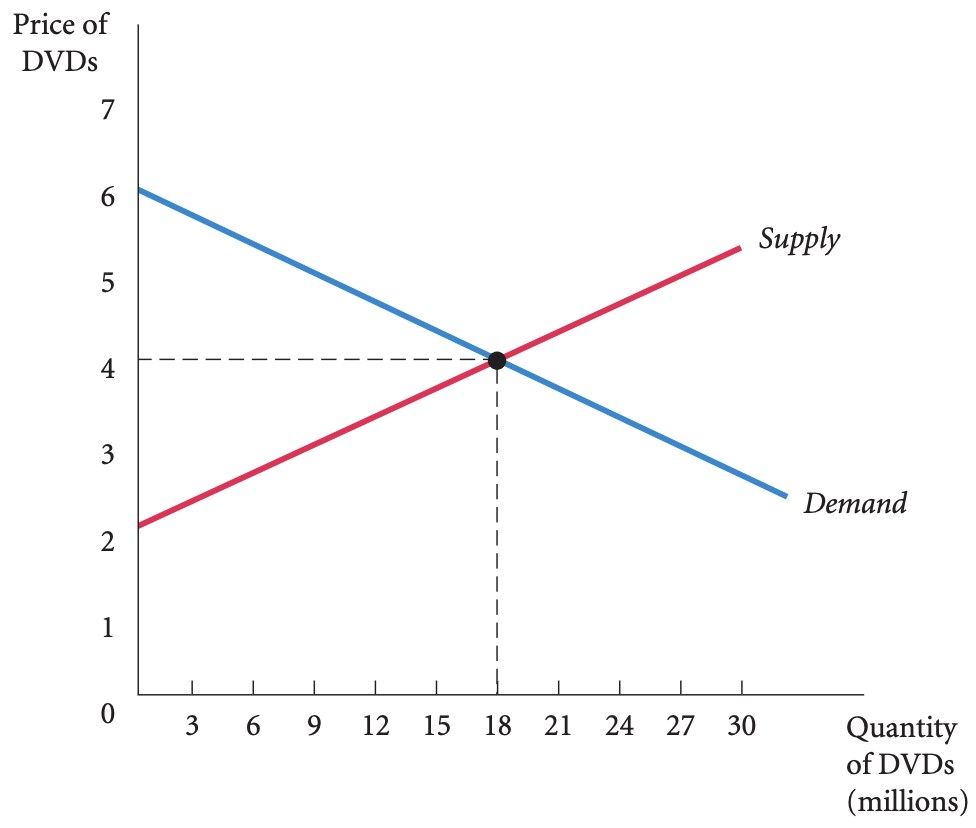
\includegraphics[width = 0.75\textwidth]{q2}
	\end{center}
	
	\begin{enumerate}
	
	\item Find the values of consumer surplus and producer surplus when the market is in equilibrium.
	
	\item If underprodution occurs in this market, and price remains \$4, but only 9 million DVDs are produced, what happens to the amounts of consumer surplus and producer surplus? What is the value of the deadweight loss?
	
	\item If overproduction occurs in this market, and price remains \$4, but 27 million DVDs are produced, what happens to the amounts of consumer surplus and producer surplus? Is there a deadweight loss with overproduction? If so, what is its value?
	
	\end{enumerate}

\item The corn lobby convinces Congress to pass a price floor on corn to boost corn farmers' earnings. Suppose demand for corn is $Q_D = 60 - 10P$ and supply is $Q_S = 5P$.

	\begin{enumerate}
	
	\item If Congress implements a price floor of \$4, how does producer surplus change?
	
	\item If Congress implements a price floor of \$5, how does producer surplus change?
	
	\end{enumerate}
	
\item The U.S. Department of Agriculture (USDA) administers the price floor for butter, which the 2008 Farm Bill set at \$2.05 per pound. At that price, according to data from the USDA, the quantity of butter supplied in 2010 was 1.7 billion pounds, and the quantity demanded was 1.6 billion pounds. To support the price of butter at the price floor, the USDA therefore had to buy up 100 million pounds of butter. The accompanying diagram shows supply and demand curves illustrating the market for butter.

	\begin{center}
	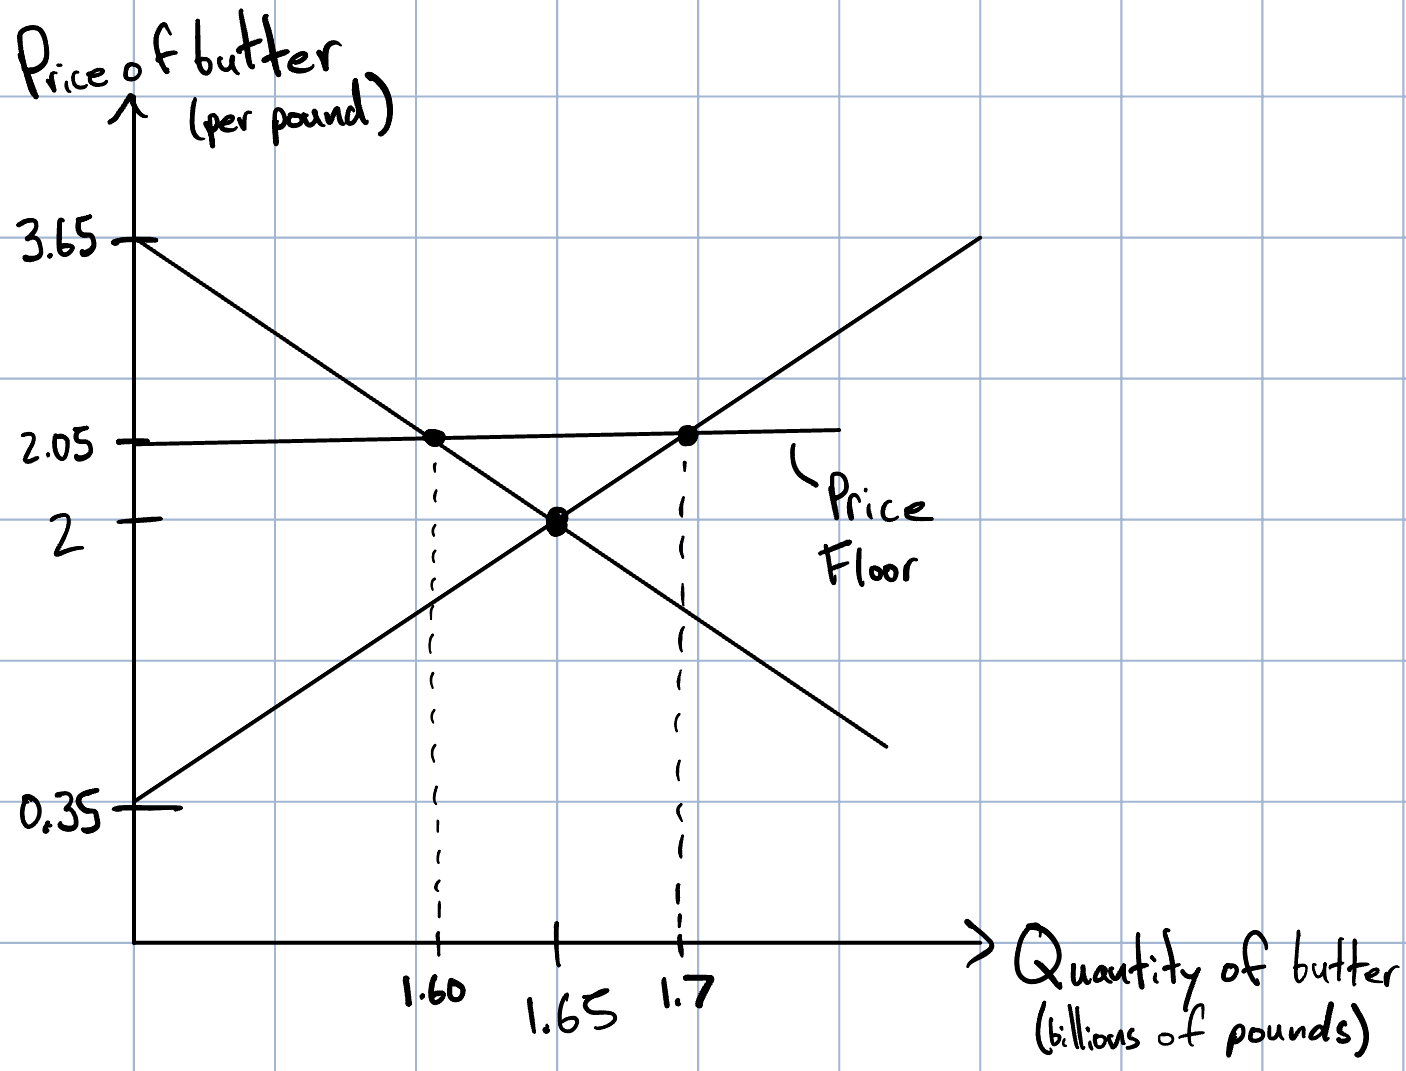
\includegraphics[width = 0.75\textwidth]{q5}
	\end{center}

	\begin{enumerate}
	
	\item In the absence of a price floor, how much consumer surplus is created? How much producer surplus? What is the total surplus?
	
	\item With the price floor at \$2.05 per pound of butter, consumers buy 1.6 billion pounds of butter. How much consumer surplus is created now?
	
	\item With the price floor at \$2.05 per pound of butter, producers sell 1.7 billion pounds of butter (some to consumers and some to the USDA). How much producer surplus is created now?
	
	\item How much money does the USDA spend on buying up surplus butter?
	
	\item Taxes must be collected to pay for the purchases of surplus butter by the USDA. As a result, total surplus is reduced by the amount the USDA spent on buying surplus butter. Using your answers for parts b-d, what is the total surplus when there is a price floor? How does this compare to the total surplus without a price floor from part a?
	
	\end{enumerate}

\end{enumerate}

\end{document}